\documentclass[11pt,a4paper]{article}
\usepackage{diagbox}
\usepackage{wrapfig}
\usepackage[utf8]{inputenc}
%\usepackage[swedish]{babel}
\usepackage{graphicx}
\usepackage{amsmath}
\usepackage{amssymb}
\usepackage{units}
\usepackage{ae}
\usepackage{icomma}
\usepackage{xcolor}
\usepackage{graphics}
\usepackage{bbm}
\usepackage{float}
\usepackage{siunitx}
\usepackage[font={small,it}]{caption}
\usepackage{subcaption}

\usepackage{hyperref}
\usepackage{epstopdf}
\usepackage{epsfig}
\usepackage{braket}
\usepackage{pdfpages}
\usepackage{tcolorbox}

\usepackage{svg}
\usepackage{physics}
% \usepackage{tikz}
% \usepackage{pgfplots}
% \pgfplotsset{compat=newest}
% \usepgfplotslibrary{groupplots}
% \usepgfplotslibrary{dateplot}

\newcommand{\N}{\ensuremath{\mathbbm{N}}}
\newcommand{\Z}{\ensuremath{\mathbbm{Z}}}
\newcommand{\Q}{\ensuremath{\mathbbm{Q}}}
\newcommand{\R}{\ensuremath{\mathbbm{R}}}
\newcommand{\C}{\ensuremath{\mathbbm{C}}}
\newcommand{\id}{\ensuremath{\,\mathrm{d}}}
\newcommand{\rd}{\ensuremath{\mathrm{d}}}
\newcommand{\Ordo}{\ensuremath{\mathcal{O}}}% Stora Ordo
\renewcommand{\L}{\ensuremath{\mathcal{L}}}% Stora Ordo
\newcommand{\sub}[1]{\ensuremath{_{\text{#1}}}}
\newcommand{\ddx}[1]{\ensuremath{ \frac{\partial}{\partial #1} }}
\newcommand{\ddxx}[2]{\ensuremath{ \frac{\partial^2}{\partial #1 \partial #2} }}
%\newcommand{\sup}[1]{\ensuremath{^{\text{#1}}}}
\newcommand*\diff{\mathop{}\!\mathrm{d}}
\renewcommand{\vec}[1]{\boldsymbol{\mathbf{#1}}}
\renewcommand{\b}[1]{\ensuremath{ {\bf #1 } }}
\renewcommand{\arraystretch}{1.5}

\title{Effect of toroidicity on runaway generation\\\vspace{.3cm} \large{project course FUF060 in plasma physics}}
\author{Peter Halldestam}
\date{\today}

\begin{document}

\maketitle

\abstract{\noindent In a tokamak plasma, \textit{runaway electrons} are created when the force from the toroidal electric field is greater than the drag force due to Coulomb collisions.
This results in an acceleration of electrons to extremely high velocities which in turn may damage components of the fusion reactor facing the plasma.
In this report we consider the cross sectional shape of the magnetic field and study its effect on runaway generation using \textsc{DREAM} (\textit{Disruption and Runaway Electron Avoidance Model}, a numerical tool primarily designed for studying the evolution of runaway electrons in tokamak disruptions \cite{DREAM}).}

\section{Parametrisation of the toroidal magnetic field}
In \textsc{DREAM}, the shape of the magnetic field is characterised by the elongation $\kappa(r)$, triangularity $\delta(r)$ and Shafranov shift $\Delta(r)$ as illustrated in fig.\ \ref{fig:toroidicity}.
Firstly, the elongation $\kappa$ is a scale factor determining the height of a flux surface in relation to the minor radius coordinate $r\in[0, a]$.
The triangularity $\delta$ determines the horizontal shift of the top-most point of the flux surface and finally, the Shafranov shift $\Delta$, which is the shift from the magnetic axis of the center of a flux surface.
These are set to be linear in $r$ such that they vanish at $r=0$ and is equal to some set value at $r=a$, ie.\ $\kappa(a)=\kappa_a$ and so on.
For instance, the configuration $(\kappa_a, \delta_a, \Delta_a)=(1, 0, 0)$ would yield a circular cross section with concentric flux surfaces.

Any position $\vec{x}$ is parametrized with the coordinates $(r, \theta)$ by defining $\vec{x}=R\vec{\hat{R}}+z\vec{\hat{z}}$, where
\begin{align}
    \label{eq:param}
    \begin{cases}
        R
        =R_0+\Delta(r)+r\cos\{\theta+\delta(r)\sin\theta\},\\
        z
        =r\kappa(r)\sin\theta.
    \end{cases}
\end{align}
With this parametrisation, each flux surface is identified by keeping $r$ constant given the major radius of the magnetic axis $R_0$ and the three shaping parameters.\\

\noindent
Furthermore, any arbitrary axisymmetric magnetic field can be expressed as
\begin{align*}
    \vec{B}
    =G\grad{\varphi}+\frac{1}{2\pi}\grad{\varphi}\cross\grad{\psi},
\end{align*}
where $\varphi$ denotes the toroidal angle about which the field is symmetric, $G$ describes the toroidal magnetic field and $\psi$ is the poloidal magnetic flux.
% The latter two are set in accordance to an example in \cite{DREAM} (REFERERA BÄTTRE)
% \begin{align*}
%     G(r)
%     &= B_0 R_0\\
%     \psi(r)
%     &=-\mu_0 I_\text{ref} \bigg[1-\bigg(\frac{r}{a}\bigg)^2\bigg] a
% \end{align*}
For our purposes, the toroidal term will dominate and therefore a useful approximation of the field strength is given by
\begin{align}
    \label{eq:magnetic}
    B
    \approx\frac{B_0 R_0}{R}
    =\frac{B_0 R_0}{R_0+r}
\end{align}
where $B_0=\SI{5}{T}$ is a prescribed value of $B=\abs{\vec{B}}$ at the major radius, ie.\ at $r=0$.
In the simulations, the major and minor radii are set to $R_0=\SI{0.68}{m}$ and $a=\SI{0.22}{m}$ respectively.
Also if nothing else is stated, the default value for the shaping parameters are $\kappa_a=1.5$, $\delta_a=0.2$ and $\Delta_a=a/10$.
% \begin{figure}[H]
%   \begin{minipage}[l]{0.6\textwidth}
%     \includesvg[scale=.55]{figs/toroidicity}
%   \end{minipage}
%   \hfill
%   \begin{minipage}[c]{0.4\textwidth}
%       \caption{\textit{Tokamak cross section illustrating the three shaping parameters used to define the shape of the magnetic field: elongation $\kappa$, triangularity $\delta$ and Shafranov shift $\Delta$.
%       This image is taken from \cite{DREAM}.}}
%       \label{fig:toroidicity}
%   \end{minipage}
% \end{figure}
\begin{figure}[H]
    \centering
    \captionsetup{width=.8\textwidth}
    \includesvg[scale=.7]{figs/toroidicity}
    \caption{Tokamak cross section illustrating the three shaping parameters used to define the shape of the magnetic field: elongation $\kappa$, triangularity $\delta$ and Shafranov shift $\Delta$.
    This image is taken from \cite{DREAM}.}
    \label{fig:toroidicity}
\end{figure}

\newpage
\section{Runaway electrons}
An electron becomes a runaway after reaching a certain speed $v>v_c$ above which the electric field becomes so strong that the accelerating electric force dominates any drag forces.
The rate at which the runaway population grows is primarily (\textcolor{red}{Finns det andra sätt?}) due to two phenomena: \textit{Dreicer generation} and \textit{Avalanche generation} \cite{embreus}.
Together, these add up to a total runaway rate of
\begin{align*}
    \dv{n_\text{re}}{t}
    =\gamma+n_\text{re}\Gamma.
\end{align*}
\textcolor{red}{Mer information om dessa fenonomen}

During a simulation in \textsc{DREAM}, the program keeps track of the runaway rate as a flux surface averaged quantity
\begin{align*}
    \expval{\dv{n_\text{re}}{t}}
    &=\frac{1}{S}\int_0^{2\pi}\diff{\varphi}\int_{-\pi}^{\pi}\diff{\theta}\mathcal{J}\dv{n_\text{re}}{t},\\
    S
    &=\int_0^{2\pi}\diff{\varphi}\int_{-\pi}^{\pi}\diff{\theta}\mathcal{J},\\
    \mathcal{J}
    &=\frac{1}{\abs{\grad{\varphi}\vdot(\grad{\theta}\cross\grad{r})}},
\end{align*}
where $S$ is the area of the surface and $\mathcal{J}$ is the spatial Jacobian of the coordinate system.

In the following section, we investigate the effect the three shaping parameters have on the electron runaway generation individually.
Firstly, without the Avalanche effect included in the simulations and solely focusing on Dreicer generation \textcolor{red}{(Är dock osäker ifall \texttt{gammaDreicer} verkligen motsvarar hela \texttt{runawaRate} i \textsc{DREAM}, med tanken på den diskrepansen vi såg för några veckor sedan när vi plottade dessa två mot varandra. Vi får diskutera detta i detalj Mathias!)},
and later including both phenomena.

\subsection{Dreicer generation}
In fig.\ \ref{fig:elongation}, the runaway rates from three different simulation with different orders of magnitude in the elongation $\kappa$ are shown to the left and an outlining of their corresponding tokamak cross sections to the right.
The elongation has seemingly no effect on the runaway generation, at least in this range of values.
Out of all three shaping parameters, this seems to be case only for $\kappa$.

Two similar analyses was performed for the triangularity $\delta$ in fig.\ \ref{fig:triangularity} and the Shafranov shift $\Delta$ in fig.\ \ref{fig:shafranovShift}.
Here we observe that cross sections with geometric centres farther away from the center of the tokamak $R=0$ tend to have less runaway electrons generated.

\begin{figure}[H]
    \centering
    \captionsetup{width=.8\textwidth}
    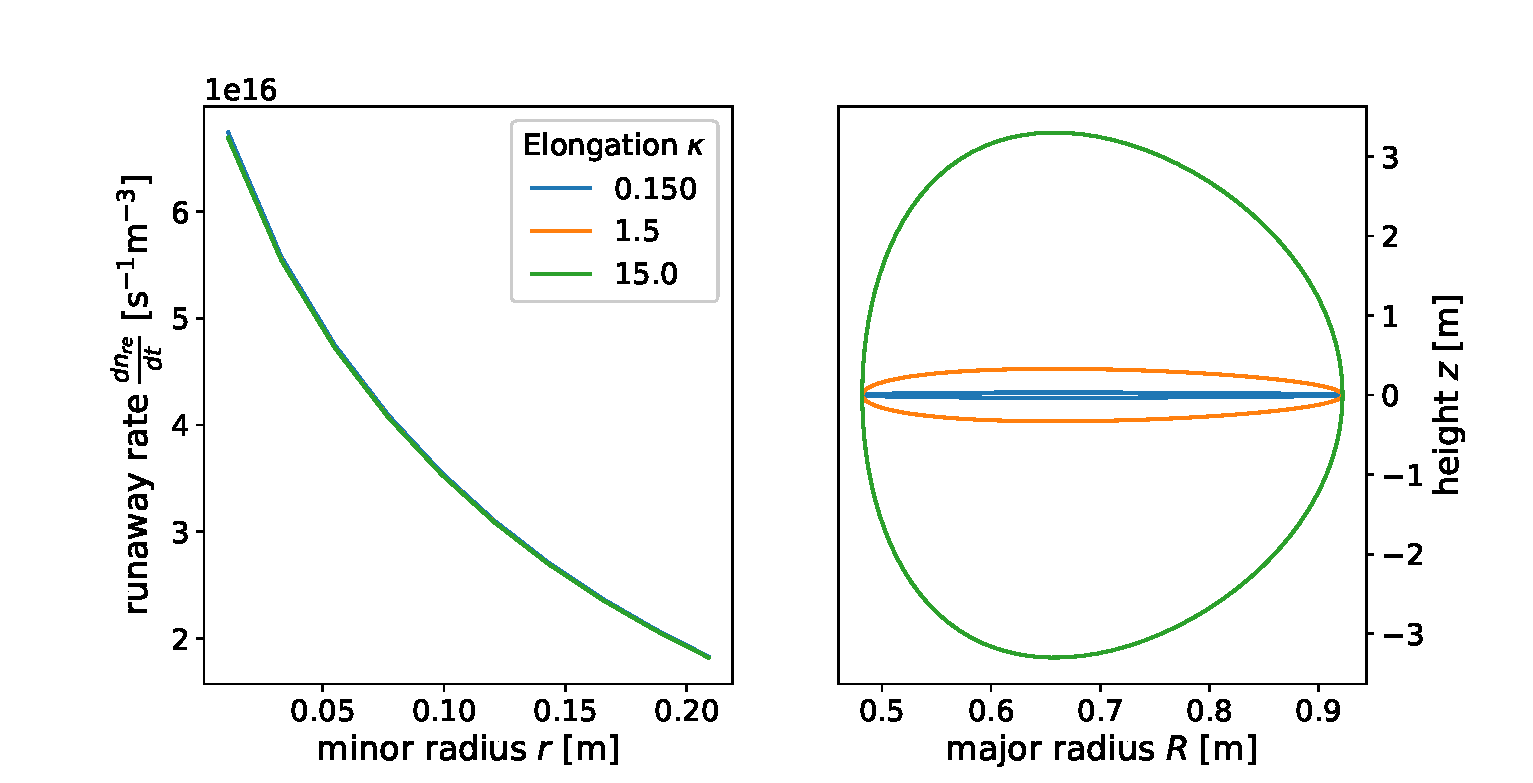
\includegraphics[width=\textwidth]{figs/elongation.eps}
    \caption{Flux surface averaged electron runaway rate $\langle\diff{n}_{re}/\diff{t}\rangle$ vs.\ minor radius coordinate $r$ for three different elongations $\kappa$ (left), and corresponding tokamak cross sections (right).
    No significant effect of $\kappa$ on the runaway rate is observed.}
    \label{fig:elongation}
\end{figure}

\begin{figure}[H]
    \centering
    \captionsetup{width=.8\textwidth}
    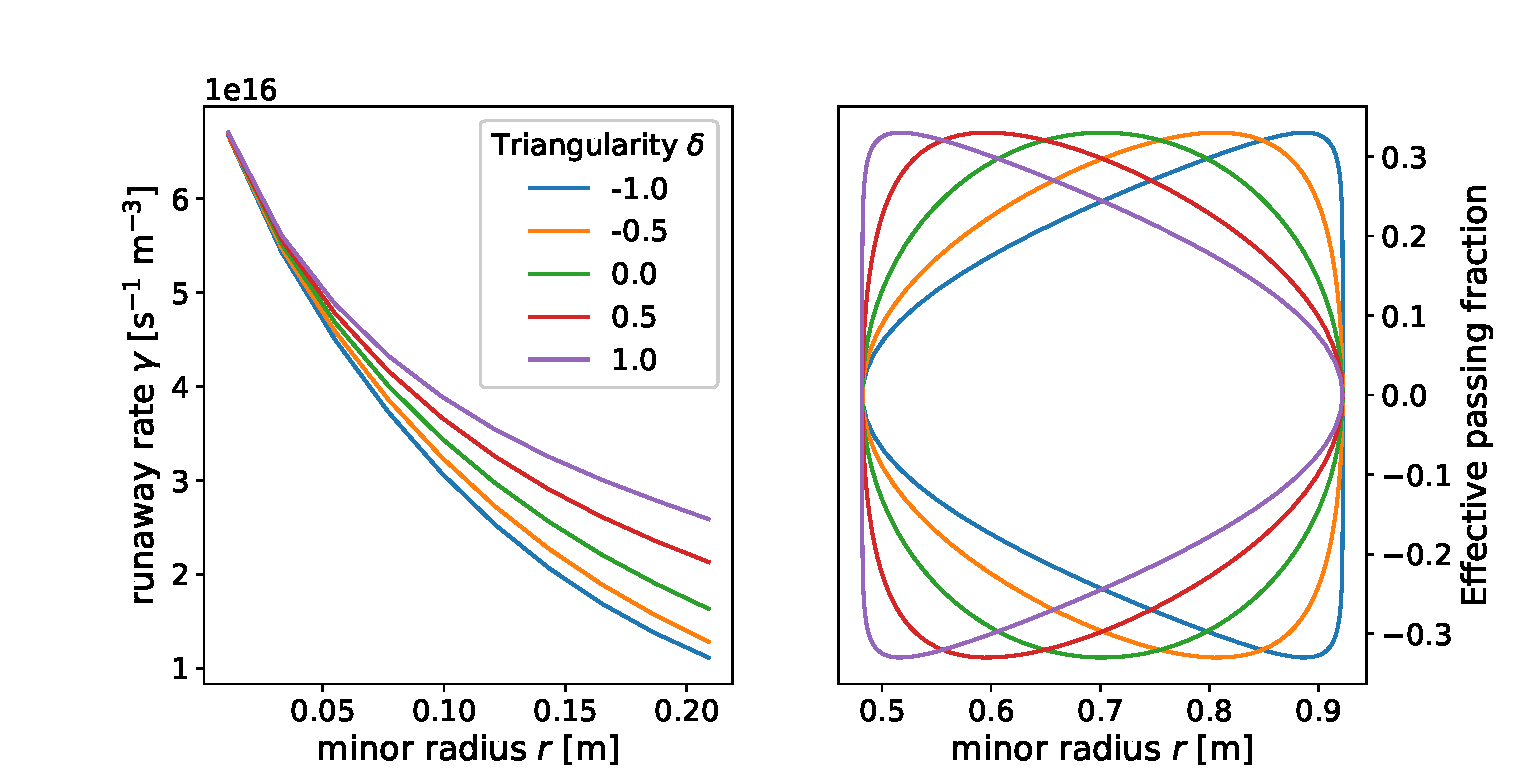
\includegraphics[width=\textwidth]{figs/triangularity.eps}
    \caption{Flux surface averaged electron runaway rate $\langle\diff{n}_{re}/\diff{t}\rangle$ vs.\ minor radius coordinate $r$ for five different triangularity $\delta$ (left), and corresponding tokamak cross sections (right).}
    \label{fig:triangularity}
\end{figure}

\begin{figure}[H]
    \centering
    \captionsetup{width=.8\textwidth}
    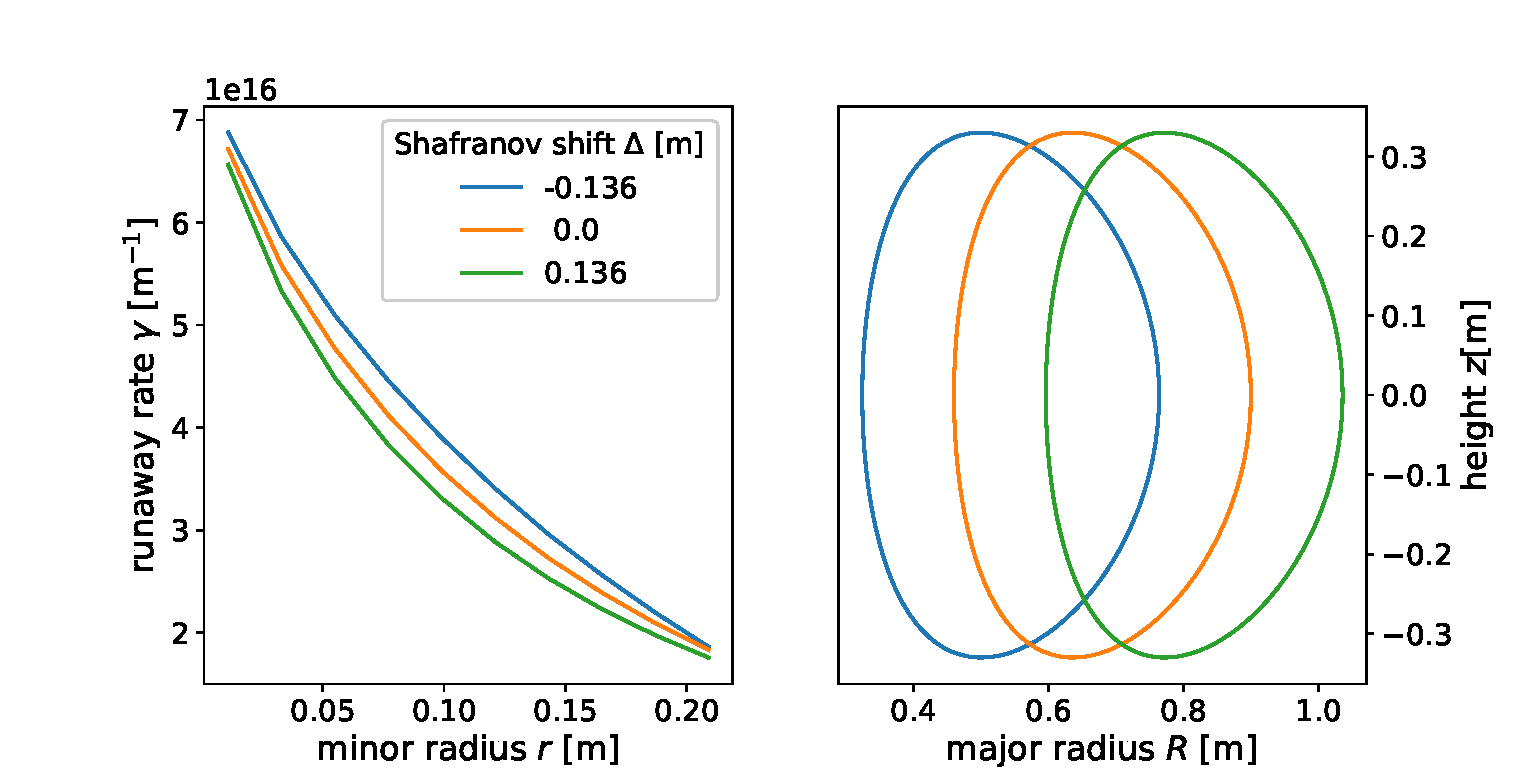
\includegraphics[width=\textwidth]{figs/shafranovShift.eps}
    \caption{Flux surface averaged electron runaway rate $\langle\diff{n}_{re}/\diff{t}\rangle$ vs.\ minor radius coordinate $r$ for three different Shafranov shifts $\Delta$ (left), and corresponding tokamak cross sections (right).}
    \label{fig:shafranovShift}
\end{figure}

\noindent
An explanation for this could possibly be the \textit{magnetic mirror effect} and the concept of \textit{trapped particles}.
Consider a charged particle with velocity components parallel $\vec{v}_\parallel$ and perpendicular $\vec{v}_\perp$ to the magnetic field, starting off at the point of its trajectory where the magnetic field strength is at its lowest $B=B_\text{min}$.
Its guiding center will \textcolor{red}{approximately?} follow a magnetic field surface and along its trajectory, the particle will experience a deaccelerating force as it moves towards higher $B$, namely
\begin{align*}
    m\dv{\vec{v}_\parallel}{t}=-\mu\grad_\parallel{B}.
\end{align*}
Here $\mu=mv_\perp^2/2B$ denotes the magnetic moment, which is an adiabatic invariant.
If the particle ever reaches $v_\parallel=0$, $v_\parallel$ will change sign and it will be forced to turn back.
It is trapped.

One can obtain a condition for a particle to be trapped based on its initial pitch $\xi_0=v_\parallel/v$ when it is at $B=B_\text{min}$ using conservation of energy \cite{hoppe}.
At any time has the total energy
\begin{align*}
    E_0
    =E_\parallel + E_\perp
    =\frac{mv_\parallel^2}{2}+\mu B
\end{align*}
The energies $E_\parallel$ and $E_\perp$ both add up the constant $E_0$, and represents the kinetic energy stored in motion parallel and perpendicular to the magnetic field surfaces respectively.
The particle is trapped if $E_\parallel$ ever reaches zero and the limiting case for this would be if it occured at the point on the surface where $B$ is at its maximum $B_\text{max}$.
In other words, it is trapped if it has a total energy
\begin{align*}
    E_0
    <\mu B_\text{max}.
\end{align*}
Due to energy conservation, we are free to evaluate $E_0$ anywhere along the trajectory and likewise for $\mu$ as it is an adiabatic invariant.
With $E_0$ evaluated where $B=B_\text{min}$ and $\mu$ where $B=B_\text{max}$, at which $v_\perp=v$ such that $\mu=mv^2/2B_\text{max}$, this inequality thus implies the following condition for a trapped particle
\begin{align*}
    \xi_0^2
    <1-\frac{B_\text{min}}{B_\text{max}}.
\end{align*}
Using the approximate expression for the magnetic field strength in eq.\ \eqref{eq:magnetic} to write $B_\text{min}/B_\text{max}=R_\text{max}/R_\text{min}$ and then parametrising $R_\text{min}$ and $R_\text{max}$ with eq.\ \eqref{eq:param} at $\theta=0$ and $\theta=\pi/2$ respectively, we obtain the following inequality for a particle to be trapped
\begin{align}
    \label{eq:condition}
    \xi_0^2
    <\frac{r[1-\sin\delta(r)]}{R_0+\Delta(r)+r}.
\end{align}
Assuming the distribution of $\xi_0$ is the same in all simulations \textcolor{red}{rimligt antagande?}, we see that \eqref{eq:condition} implies firstly that for small negative values of $\delta$, more particles will be trapped than for small positive values.
This conclusion fits rather well with what is observed in fig.\ \ref{fig:triangularity}, as trapped particles are unable to turn into runaways \textcolor{red}{behövs förklaring?} effectively reducing the runaway generation rate.
Secondly, an increased $\Delta$ would result in the contrary: fewer trapped particles, which also fits the observation from fig.\ \ref{fig:shafranovShift}.

\subsection{Avalanche generation}
\textcolor{red}{inkludera Avalanche i motsvarande simuleringar.}

\begin{thebibliography}{100}
    \bibitem{DREAM}
    DREAM documentation, \url{https://ft.nephy.chalmers.se/dream/index.html} (accessed 21/9/21)

    \bibitem{embreus}
    O.\ Embréus, \textit{Kinetic modelling of runaway in plasmas}, PhD thesis, Chalmers University of Technology, Göteborg (2019)

    \bibitem{hoppe}
    M.\ Hoppe, \textit{Simulation of charged particle orbits in fusion plasma}, BSc thesis, Chalmers University of Technology, Göteborg (2015)

\end{thebibliography}




\end{document}
